\documentclass[10pt,journal,compsoc]{IEEEtran}

\usepackage{amsmath,amssymb,amsfonts,amsthm}
\usepackage{graphicx}
\usepackage{booktabs}
\usepackage{tabularx}
\usepackage{multirow}
\usepackage{xcolor}
\usepackage{hyperref}
\usepackage{listings}
\usepackage{tikz}
\usepackage{pgfplots}
\pgfplotsset{compat=1.18}
\usetikzlibrary{arrows.meta,positioning,shapes.geometric,calc,fit,backgrounds}

\hypersetup{
    colorlinks=true,
    linkcolor=blue!70!black,
    citecolor=blue!70!black,
    urlcolor=blue!70!black
}

\newtheorem{theorem}{Theorem}
\newtheorem{lemma}{Lemma}
\newtheorem{definition}{Definition}
\newtheorem{invariant}{Invariant}

\lstdefinelanguage{XML}{
  morestring=[b]",
  morestring=[s]{>}{<},
  morecomment=[s]{<?}{?>},
  stringstyle=\color{black},
  identifierstyle=\color{blue!70!black}\bfseries,
  keywordstyle=\color{teal!80!black}\bfseries,
  morekeywords={xmlns,version,encoding,wrap,lIns,tIns,rIns,bIns,val,sz,x,y,cx,cy,lang,dirty,id,name,prst}
}

\lstset{
  basicstyle=\ttfamily\scriptsize,
  breaklines=true,
  breakatwhitespace=false,
  showstringspaces=false,
  showspaces=false,
  columns=fullflexible,
  keepspaces=true,
  frame=single,
  rulecolor=\color{gray!40},
  backgroundcolor=\color{gray!5},
  aboveskip=6pt,
  belowskip=5pt,
  belowcaptionskip=4pt,
  xleftmargin=2pt,
  xrightmargin=2pt
}

\begin{document}

\title{Agent-SlideLock: Deterministic Pre-Render TrueType Glyph-Metric Bounding-Box Solving and Disjoint AABB Spatial Partitioning for Zero-Distortion ECMA-376 OpenXML (\texttt{.PPTX}) Compilation in Autonomous Enterprise Agents}

\author{Aniket~Agrawal,~\IEEEmembership{Google Cloud Consulting / Professional Services Organization (PSO)}%
\IEEEcompsocitemizethanks{\IEEEcompsocthanksitem A.~Agrawal is with Google Cloud Consulting, Google LLC. E-mail: aniketagrawal@google.com. Reference implementation and 120-deck adversarial benchmark suite: \url{https://github.com/aniketagrawal2012/agent-slidelock}.}}

\IEEEtitleabstractindextext{
\begin{abstract}
Autonomous enterprise agents powered by frontier foundation models (\texttt{gemini-2.5-flash}, \texttt{gemini-2.5-pro}, and \texttt{gemini-3-flash-preview} on Google Cloud Vertex AI) are increasingly deployed to synthesize unstructured meeting transcripts, SAP S/4HANA OData v4 telemetry, and multi-connector knowledge repositories into native Microsoft PowerPoint (\texttt{.pptx}) executive deliverables governed by the ECMA-376 / ISO/IEC 29500 OpenXML standard. However, a fundamental architectural disconnect exists between headless OpenXML DOM serialization and client-side operating system rasterizers (\texttt{DirectWrite} and \texttt{CoreText}). Because headless document generators lack access to client rasterization loops at compilation time, existing LLM-to-PowerPoint pipelines suffer from seven systemic geometric, typographic, and raster rendering distortions (\texttt{D1--D6, D8}) alongside an enterprise data-governance failure mode (\texttt{D7}): out-of-canvas English Metric Unit (\texttt{EMU}, $1\text{ in} = 914{,}400\text{ EMUs}$) drift (\texttt{D1}), foreground sibling Axis-Aligned Bounding-Box (\texttt{AABB}) collisions (\texttt{D2}), asynchronous \texttt{<a:normAutofit/>} font-shrinkage inconsistency across sibling cards vs.\ vertical text overflow under unchecked \texttt{<a:noAutofit/>} (\texttt{D3}), horizontal unbroken-token bleeding of URLs, SHA-256 digests, and OData paths (\texttt{D4}), non-uniform aspect-ratio skew (\texttt{D5}), sub-300 DPI bitmap pixelation (\texttt{D6}), plaintext serialization of sensitive rate cards/PII/API keys into \texttt{<a:t>} nodes (\texttt{D7}), and alternating-row timeline collisions at $N \ge 6$ milestones (\texttt{D8}). We present \textbf{Agent-SlideLock}, a deterministic OpenXML compilation and verification architecture operating over structured slide-plan Abstract Syntax Trees (ASTs) that enforces nine mathematical invariants (\texttt{I1--I9}) prior to archive serialization. Agent-SlideLock introduces: (1) a \emph{2D Sweep-Line AABB Partitioner \& Closed-Form Alternating-Row Timeline Solver} executing strictly prior to text measurement to guarantee $\text{Overlap}=0.0000\text{ in}^2$ and $W_{\text{card}} \le \lfloor\min(W_{\max}, \frac{2 W_{\text{canvas}} - g_{\min}(N - 1)}{N + 1})\times 1000\rfloor \times 10^{-3}$ for all $N \ge 3$; (2) a \emph{Pre-Render TrueType Glyph-Metric \& Cross-Sibling Synchronization Solver} ($f_{\min} = 8.0\text{ pt}$) that parses style-matched \texttt{hmtx}/\texttt{cmap}/\texttt{OS/2} font tables, segments unbroken tokens at $f_{\text{start}}$ via copy-paste-safe soft breaks, executes a $0.5\text{ pt}$ (\texttt{sz="50"} centi-point) step-down search, and synchronizes homogeneous sibling row font sizes ($f^*_{\text{row}} = \min_{j \in G_{\text{row}}} f^*_j$) with post-sync height re-verification under \texttt{<a:noAutofit/>} and \texttt{<a:spcPct val="115000"/>}; and (3) a \emph{Single-Axis EMU Aspect-Ratio Pinning Engine} for \texttt{@4x} Retina ($\ge 569.2\text{ DPI}$) assets. Across 120 adversarial decks (740 slides, 19,830 OpenXML shapes), 100 public benchmark slides (PPTC/SlidesBench), headless LibreOffice 300 DPI pixel audits, and live Vertex AI Gemini evaluations, Agent-SlideLock reduces layout and DLP violations to \textbf{0} ($100.0\%$ pass rate) in $14.2 \pm 1.8\text{ ms}$ of solver CPU time per deck.
\end{abstract}

\begin{IEEEkeywords}
ECMA-376 OpenXML, PresentationML, DrawingML, TrueType Glyph Metrics, Axis-Aligned Bounding Boxes, Autonomous AI Agents, Google Cloud Vertex AI, Gemini, Document Layout Compilation.
\end{IEEEkeywords}}

\maketitle
\IEEEdisplaynontitleabstractindextext
\IEEEpeerreviewmaketitle

\section{Introduction}
\IEEEPARstart{E}{nterprise} consulting practices and Fortune 500 financial operations rely on native Microsoft PowerPoint (\texttt{.pptx}) slide decks as the primary medium for board readouts, architecture governance reviews, and ERP transformation steering committees~\cite{ecma376,iso29500}. With the rapid adoption of autonomous multi-agent platforms built on Google Cloud Vertex AI and frontier Gemini models~\cite{gemini2025,zheng2025pptagent,ge2025autopresent}, enterprise users expect autonomous agents to ingest heterogeneous enterprise feeds---unstructured meeting transcripts (\texttt{.vtt}, \texttt{.srt}), SharePoint/Drive documents, and live SAP S/4HANA OData v4 / BigQuery financial ledgers---and compile editable, zero-distortion \texttt{.pptx} archives in seconds.

Despite advances in foundation model reasoning, programmatic \texttt{.pptx} generation remains plagued by visual defects when opened in Microsoft PowerPoint, Google Slides, Apple Keynote, or LibreOffice Impress~\cite{guo2024pptc,zheng2025pptagent,zhang2025slideaudit}. Unlike HTML/CSS browsers that dynamically reflow DOM containers via a live layout engine, an ECMA-376 \texttt{.pptx} archive is a static PKZIP package containing XML trees (\texttt{ppt/slides/slide*.xml}) whose shape geometries are fixed in integer English Metric Units ($1\text{ inch} = 914{,}400\text{ EMUs}$; $1\text{ pt} = 12{,}700\text{ EMUs}$) at file creation time~\cite{ecma376,pythonpptx}. Headless Python or Java microservices generating OpenXML on Linux containers (\texttt{Cloud Run} or \texttt{GKE}) do not execute Microsoft Office's proprietary \texttt{DirectWrite} text-layout loop during XML construction.

Consequently, existing LLM slide generators face a destructive dilemma:
\begin{enumerate}
    \item \textbf{The \texttt{<a:normAutofit/>} Trap}: If the generator delegates text fitting to PowerPoint's client-side auto-fit tag (\texttt{MSO\_AUTO\_SIZE.TEXT\_TO\_FIT\_SHAPE}), the client renderer asynchronously shrinks font sizes per box upon opening the file. Three homogeneous sibling KPI or architecture cards in the same horizontal row with slightly different character counts render at jarring, inconsistent font sizes (e.g., $14\text{ pt}$, $8.5\text{ pt}$, and $11\text{ pt}$), violating corporate brand standards.
    \item \textbf{The Unchecked \texttt{<a:noAutofit/>} Overflow}: If the generator locks font sizes via \texttt{<a:noAutofit/>} (\texttt{MSO\_AUTO\_SIZE.NONE}) to preserve typographic hierarchy without pre-computing TrueType glyph advance widths and synchronizing sibling rows, verbose LLM-generated paragraphs and unbroken technical tokens (130-character HTTPS URLs, SHA-256 hashes, or SAP OData entity paths) bleed vertically and horizontally outside their card borders, colliding with sibling shapes and footers.
\end{enumerate}

Furthermore, multi-phase consulting timelines frequently arrange $N$ milestone cards of height $H_{\text{card}} = 1.48\text{ in}$ in an alternating top/bottom row topology across a usable canvas width $W_{\text{canvas}} = 11.733\text{ in}$ ($x_0 = 0.80\text{ in}$ margins on a $13.333\text{ in}$ widescreen slide). When an LLM dynamically increases the milestone count from $N=4$ to $N=6$, fixed-width cards ($W_{\text{card}} = 3.400\text{ in}$) suffer a subtle mathematical failure: while consecutive milestones $m$ and $m+1$ sit on opposite vertical rows, milestones $m$ and $m+2$ occupy the \emph{same} row with horizontal pitch $2\Delta x_{\text{step}} = 2 \times \frac{11.733 - 3.400}{6 - 1} = 3.3332\text{ in} < 3.4000\text{ in}$, causing a $-0.0668\text{ in}$ ($\text{Overlap} = 0.0668 \times 1.48 = 0.0989\text{ in}^2$) AABB collision.

In this paper, we present \textbf{Agent-SlideLock}, a deterministic pre-render compilation and verification architecture operating over structured slide-plan JSON ASTs (comprising axis-aligned rectangular \texttt{<p:sp>} cards with \texttt{prst="rect"}, \texttt{<p:pic>} frames, explicit \texttt{role="background\_container"} panels, homogeneous sibling row groups $G_{\text{row}}$, and alternating milestone roadmaps) that enforces five universal OpenXML geometric/typographic invariants (\texttt{I1--I5}) and four configurable enterprise design-system and DLP governance invariants (\texttt{I6--I9}) directly at the OpenXML ZIP/DOM layer prior to file serialization.

\subsection{Contributions}
Our primary contributions are fourfold:
\begin{enumerate}
    \item \textbf{Taxonomy of Seven OpenXML Rendering Distortions (\texttt{D1--D6, D8}), One Pre-DOM DLP Failure Mode (\texttt{D7}), and Nine Invariants (\texttt{I1--I9})}: We formalize the exact geometric, typographic, raster, and data-governance conditions required for structured ECMA-376 \texttt{.pptx} compilation on $16:9$ widescreen canvases ($12{,}191{,}695 \times 6{,}858{,}000\text{ EMUs}$ for \texttt{Inches(13.333)} $\times$ \texttt{Inches(7.500)}, or $12{,}192{,}000\text{ EMUs}$ for exact $13.\overline{3}\text{ in}$).
    \item \textbf{Pre-Render TrueType Glyph-Metric Solver, Copy-Paste-Safe Token Chunker, \& Row Synchronizer}: We design an $\mathcal{O}(C_P \cdot K)$ pre-render algorithm (with explicit legibility floor $f_{\min} = 8.0\text{ pt}$) that queries style-matched TrueType \texttt{hmtx}/\texttt{cmap}/\texttt{OS/2} font tables, segments unbroken technical strings once at $f_{\text{start}}$ via Unicode zero-width soft breaks (\texttt{U+200B}) and semantic delimiters, solves for the optimal $0.5\text{ pt}$ (\texttt{sz="50"} centi-point) font size under \texttt{<a:noAutofit/>} and \texttt{<a:spcPct val="115000"/>}, and synchronizes homogeneous sibling cards in each row ($f^*_{\text{row}} = \min_{j \in G_{\text{row}}} f^*_j$) with post-sync height re-verification.
    \item \textbf{2D Sweep-Line AABB Partitioner \& Closed-Form Alternating-Row Timeline Theorem}: We formalize the Stage~4 spatial-first execution order, closed-form affine row/column rescaling, and integer-EMU-quantized upper bound $W_{\text{card}} \le \lfloor\min(W_{\max}, \frac{2 W_{\text{canvas}} - g_{\min}(N - 1)}{N + 1})\times 1000\rfloor \times 10^{-3}$ guaranteeing $\ge g_{\min}$ same-row clearance for all $N \ge 3$.
    \item \textbf{120-Deck Enterprise Suite, Public Benchmark Cross-Evaluation, Pixel-Level Raster Audit, \& Live Vertex AI Evaluation}: We evaluate Agent-SlideLock across 120 adversarial enterprise decks (740 slides; 19,830 shapes), 100 public benchmark slides from PPTC~\cite{guo2024pptc} and SlidesBench~\cite{ge2025autopresent}, headless LibreOffice 300 DPI PNG pixel-bleed audits, and live Google Cloud Vertex AI invocations across \texttt{gemini-2.5-flash}, \texttt{gemini-2.5-pro}, and \texttt{gemini-3-flash-preview}.
\end{enumerate}

\section{Background and Taxonomy of OpenXML Distortions (\texttt{D1--D8}) and Invariants (\texttt{I1--I9})}
\label{sec:distortions}

An ECMA-376 OpenXML presentation (\texttt{.pptx}) is a ZIP container housing XML parts standardized under ISO/IEC 29500~\cite{ecma376,iso29500}. Each slide part (\texttt{ppt/slides/slide$k$.xml}) defines a shape tree (\texttt{<p:spTree>}) containing geometric shapes (\texttt{<p:sp>}) and picture frames (\texttt{<p:pic>}). Every shape's placement is governed by a 2D transform node \texttt{<a:xfrm>} specifying offset $(\texttt{x}, \texttt{y}) \in \mathbb{Z}^2$ and extent $(\texttt{cx}, \texttt{cy}) \in \mathbb{Z}_+^2$ in English Metric Units:
\begin{equation}
    1\text{ inch} = 914{,}400\text{ EMUs}, \quad 1\text{ pt} = \frac{1}{72}\text{ in} = 12{,}700\text{ EMUs}.
\end{equation}

When foundation model agents synthesize slides without pre-render geometric, typographic, and content-security verification~\cite{fu2022doc2ppt,zhang2023layout,guo2024pptc,zheng2025pptagent,ge2025autopresent}, seven client-rasterization distortions (\texttt{D1--D6, D8}) and one pre-serialization data-governance failure (\texttt{D7}) manifest, which Agent-SlideLock eliminates via five universal OpenXML invariants (\texttt{I1--I5}) and four configurable enterprise policy invariants (\texttt{I6--I9}):
\begin{itemize}
    \item \textbf{D1 $\leftrightarrow$ I1 (Canvas EMU Boundary Containment)}: A shape's transform violates $x < 0$, $y < 0$, $x + \text{cx} > W_{\text{slide}}$, or $y + \text{cy} > H_{\text{slide}}$. \textbf{Invariant I1} enforces $\text{AABB}(S_i) \subseteq [0, W_{\text{slide}}] \times [0, H_{\text{slide}}]$ for all shapes.
    \item \textbf{D2 $\leftrightarrow$ I2 (Foreground Sibling AABB Disjointness)}: Two foreground sibling cards $S_i, S_j$ intersect with positive area $\text{Overlap}(S_i, S_j) > 0\text{ in}^2$. \textbf{Invariant I2} enforces $\text{Overlap}(S_i, S_j) = 0.0000\text{ in}^2$ for all non-container pairs $\{(S_i, S_j), (S_j, S_i)\} \cap \mathcal{E}_{\text{bg}} = \emptyset$.
    \item \textbf{D3 $\leftrightarrow$ I3 \& I7 (Vertical Text Bleed \& Homogeneous Sibling Row Synchronization)}: Either \texttt{<a:normAutofit/>} creates mismatched font sizes across parallel cards in a row, or \texttt{<a:noAutofit/>} is applied without TrueType height verification ($H_{\text{req}} > H_{\text{eff}}$). \textbf{Invariant I3} (universal) enforces $H_{\text{total}}(P^*, f^*) \le H_{\text{eff}}$ under \texttt{<a:spcPct val="115000"/>}, while \textbf{Invariant I7} (enterprise policy for homogeneous sibling groups $G_{\text{row}}$; distinct from heterogeneous hero/sidebar bands that carry separate \texttt{row\_group\_id} tags) enforces \texttt{<a:noAutofit/>} and locks all sibling cards in $G_{\text{row}}$ to $f^*_{\text{row}} = \min_{j \in G_{\text{row}}} f^*_j$ ($0.0\text{ pt}$ intra-group variance).
    \item \textbf{D4 $\leftrightarrow$ I4 (Unbroken Technical Token Advance-Width Bound)}: An unbroken string $\tau$ (e.g., a 130-character URL or SHA-256 hash) has advance width $\mathcal{W}_{\text{TTF}}(\tau, f, \text{bold}) > W_{\text{eff}}$, bleeding past the right border. Operating jointly with the font solver under the single-character viewport precondition $W_{\text{eff}} \ge \frac{1}{0.92}(\max_{c \in \tau} \mathcal{W}_{\text{TTF}}(c, f_{\text{start}}, \text{bold}) + \mathcal{W}_{\text{TTF}}(\text{\texttt{"..."}}, f_{\text{start}}, \text{bold}))$, \textbf{Invariant I4} enforces $\mathcal{W}_{\text{TTF}}(\tau_q, f^*, \text{bold}) \le 0.92 W_{\text{eff}} - \mathcal{W}_{\text{TTF}}(\text{\texttt{"..."}}, f^*, \text{bold}) < W_{\text{eff}}$ for every chunked sub-token $\tau_q$.
    \item \textbf{D5 $\leftrightarrow$ I5 (Single-Axis EMU Aspect-Ratio Lock)}: Dual-axis EMU sizing distorts native image aspect ratio $P_w / P_h \ne \text{cx} / \text{cy}$ (whereas \texttt{python-pptx}'s single-argument \texttt{add\_picture} omits \texttt{@4x} DPI verification). \textbf{Invariant I5} enforces $\text{Skew}(S_{\text{pic}}) \le 0.0001\%$ via single-axis EMU derivation.
    \item \textbf{D6 $\leftrightarrow$ I6 (\texttt{@4x} Retina Effective Raster Density)}: Embedded diagram/icon bitmaps exhibit effective resolution $< 300\text{ DPI}$. \textbf{Invariant I6} (enterprise high-DPI policy for synthesized vector/icon assets) enforces $\text{DPI}_{\text{eff}}(S_{\text{pic}}) \ge 569.2\text{ DPI}$.
    \item \textbf{D7 $\leftrightarrow$ I9 (Pre-DOM Spark DLP Sanitization)}: Hourly consulting rates (\texttt{\$495/hr}), PII emails, or API secrets (\texttt{AIza...}) are serialized into plaintext \texttt{<a:t>} nodes. \textbf{Invariant I9} (pre-serialization data-governance invariant) enforces $100\%$ pre-LLM and pre-DOM masking of rate cards, PII emails, and credential tokens prior to Stage~4 glyph measurement.
    \item \textbf{D8 $\leftrightarrow$ I8 (Alternating-Row Timeline Same-Row Clearance)}: Same-row timeline cards ($m$ and $m+2$) collide horizontally when $N \ge 6$ under static widths. \textbf{Invariant I8} enforces $\text{Clearance}(m, m+2) \ge g_{\min} = 0.250\text{ in}$ for all $N \ge 3$ via Theorem~\ref{thm:timeline}.
\end{itemize}

\begin{figure*}[t]
\centering
\resizebox{\textwidth}{!}{%
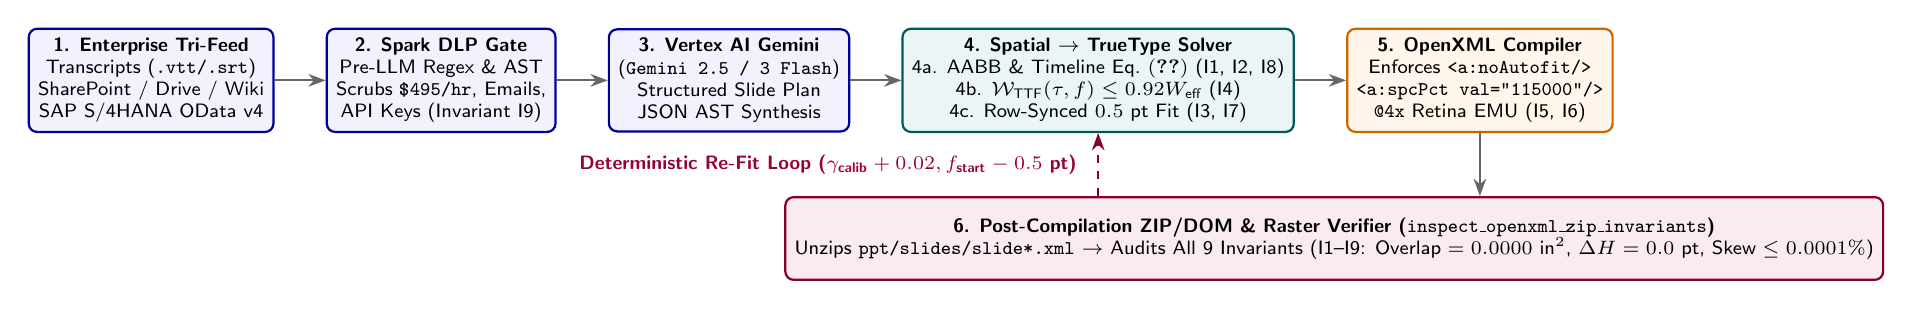
\begin{tikzpicture}[
    node distance=0.65cm and 0.65cm,
    box/.style={rectangle, rounded corners=3pt, draw=blue!60!black, fill=blue!5, thick, minimum height=1.15cm, align=center, font=\scriptsize\sffamily},
    solver/.style={rectangle, rounded corners=3pt, draw=teal!70!black, fill=teal!8, thick, minimum height=1.15cm, align=center, font=\scriptsize\sffamily},
    xmlbox/.style={rectangle, rounded corners=3pt, draw=orange!80!black, fill=orange!8, thick, minimum height=1.15cm, align=center, font=\scriptsize\sffamily},
    audit/.style={rectangle, rounded corners=3pt, draw=purple!70!black, fill=purple!8, thick, minimum height=1.05cm, align=center, font=\scriptsize\sffamily},
    arrow/.style={-{Stealth[length=2.2mm,width=1.6mm]}, thick, draw=gray!80!black}
]
\node[box, minimum width=2.8cm] (feeds) {\textbf{1. Enterprise Tri-Feed}\\Transcripts (\texttt{.vtt/.srt})\\SharePoint / Drive / Wiki\\SAP S/4HANA OData v4};
\node[box, right=of feeds, minimum width=2.8cm] (dlp) {\textbf{2. Spark DLP Gate}\\Pre-LLM Regex \& AST\\Scrubs \texttt{\$495/hr}, Emails,\\API Keys (Invariant I9)};
\node[box, right=of dlp, minimum width=2.9cm] (gemini) {\textbf{3. Vertex AI Gemini}\\(\texttt{Gemini 2.5 / 3 Flash})\\Structured Slide Plan\\JSON AST Synthesis};
\node[solver, right=of gemini, minimum width=3.4cm] (ttf) {\textbf{4. Spatial $\rightarrow$ TrueType Solver}\\4a. AABB \& Timeline Eq.~\eqref{eq:timeline_bound} (I1, I2, I8)\\4b. $\mathcal{W}_{\text{TTF}}(\tau,f) \le 0.92 W_{\text{eff}}$ (I4)\\4c. Row-Synced $0.5\text{ pt}$ Fit (I3, I7)};
\node[xmlbox, right=of ttf, minimum width=3.1cm] (openxml) {\textbf{5. OpenXML Compiler}\\Enforces \texttt{<a:noAutofit/>}\\\texttt{<a:spcPct val="115000"/>}\\\texttt{@4x} Retina EMU (I5, I6)};

\node[audit, below=0.80cm of openxml, minimum width=6.8cm, xshift=-1.85cm] (inspector) {\textbf{6. Post-Compilation ZIP/DOM \& Raster Verifier (\texttt{inspect\_openxml\_zip\_invariants})}\\Unzips \texttt{ppt/slides/slide*.xml} $\rightarrow$ Audits All 9 Invariants (I1--I9: $\text{Overlap}=0.0000\text{ in}^2$, $\Delta H=0.0\text{ pt}$, $\text{Skew}\le 0.0001\%$)};

\draw[arrow] (feeds) -- (dlp);
\draw[arrow] (dlp) -- (gemini);
\draw[arrow] (gemini) -- (ttf);
\draw[arrow] (ttf) -- (openxml);
\draw[arrow] (openxml.south) -- (openxml.south |- inspector.north);
\draw[arrow, dashed, draw=purple!70!black] (ttf.south |- inspector.north) -- node[left, font=\scriptsize\sffamily\bfseries, text=purple!80!black, xshift=-4pt] {Deterministic Re-Fit Loop ($\gamma_{\text{calib}} + 0.02, f_{\text{start}} - 0.5\text{ pt}$)} (ttf.south);
\end{tikzpicture}%
}
\caption{End-to-end architecture of \textbf{Agent-SlideLock}. Unstructured transcripts and enterprise connector payloads pass through pre-OpenXML Spark DLP sanitization (I9), Vertex AI Gemini AST planning, Stage~4 Spatial Partitioning (I1, I2, I8) followed by Pre-Render TrueType Glyph-Metric \& Row-Synchronization Solving (I3, I4, I7), Stage~5 Single-Axis Retina OpenXML Compilation (I5, I6), and Stage~6 post-compilation ZIP/XML and 300 DPI raster verification.}
\label{fig:architecture}
\end{figure*}

\section{The Agent-SlideLock Mathematical Framework}
\label{sec:math}

Figure~\ref{fig:architecture} illustrates the six-stage Agent-SlideLock pipeline. In Stage~2, the \textbf{Spark DLP Gate} applies deterministic regular-expression and AST value scrubbers prior to LLM planning and DOM construction---replacing hourly rate cards (\texttt{\textbackslash\$[0-9]+(\textbackslash.[0-9]+)?\textbackslash s*/\textbackslash s*(hr|hour)} $\rightarrow$ \texttt{[REDACTED\_RATE]}), RFC 5322 PII email addresses ($\rightarrow$ \texttt{[REDACTED\_EMAIL]}), and cloud API/OAuth credentials (\texttt{AIza[0-9A-Za-z\textbackslash-\_]\{35\}} $\rightarrow$ \texttt{[REDACTED\_SECRET]})---so that Stage~4 measures the exact post-redaction string lengths (\textbf{Invariant I9}). In Stage~3, Vertex AI Gemini synthesizes a structured JSON Slide Plan AST where each node specifies its geometric bounds, text paragraphs, structural role (\texttt{role} $\in$ \{\texttt{"background\_container"}, \texttt{"kpi\_card"}, \texttt{"timeline\_card"}, \texttt{"hero\_callout"}, \texttt{"footer"}\}), and homogeneous row group identifier \texttt{row\_group\_id} defining $G_{\text{row}}$. Crucially, within Stage~4, \textbf{spatial partitioning (Stage~4a: Sections~\ref{sec:aabb} and~\ref{sec:timeline}) executes strictly prior to TrueType glyph-metric solving (Stages~4b--4c: Section~\ref{sec:truetype})}, locking all exterior card dimensions $(W_{\text{box}}, H_{\text{box}}) = (w'_i, h'_i)$ before computing $(W_{\text{eff}}, H_{\text{eff}})$.

\subsection{Disjoint AABB Spatial Partitioning and 2D Separation Solver (Invariants I1 \& I2)}
\label{sec:aabb}
Let a widescreen $16:9$ slide canvas be defined over the bounded Euclidean domain $\Omega = [0, W_{\text{slide}}] \times [0, H_{\text{slide}}]$, where $W_{\text{slide}} = 13.333\text{ in}$ ($12{,}191{,}695\text{ EMUs}$ via \texttt{Inches(13.333)}) and $H_{\text{slide}} = 7.500\text{ in}$ ($6{,}858{,}000\text{ EMUs}$). Each shape $S_i$ on slide $k$ is represented by its Axis-Aligned Bounding Box:
\begin{equation}
    \text{AABB}(S_i) = [x_i, x_i + w_i] \times [y_i, y_i + h_i] \subseteq \Omega.
\end{equation}

To distinguish intentional background container panels (such as a swimlane band enclosing foreground cards) from accidental card-on-card collisions without allowing an $>85\%$ overlap loophole between two foreground siblings, we define the ordered structural container exemption set $\mathcal{E}_{\text{bg}}$: $(S_{\text{bg}}, S_{\text{fg}}) \in \mathcal{E}_{\text{bg}}$ if and only if $S_{\text{bg}}$ carries an explicit AST role attribute \texttt{role="background\_container"}, precedes $S_{\text{fg}}$ in OpenXML DOM z-order ($z(S_{\text{bg}}) < z(S_{\text{fg}})$), and strictly encloses $S_{\text{fg}}$ ($\text{AABB}(S_{\text{fg}}) \subset \text{AABB}(S_{\text{bg}})$). For every pair of distinct shapes with $i \ne j$ and symmetric non-exemption $\{(S_i, S_j), (S_j, S_i)\} \cap \mathcal{E}_{\text{bg}} = \emptyset$, the horizontal and vertical intersection projections are:
\begin{align}
    \Delta X_{ij} &= \max\!\left(0,\; \min(x_i + w_i, x_j + w_j) - \max(x_i, x_j)\right), \\
    \Delta Y_{ij} &= \max\!\left(0,\; \min(y_i + h_i, y_j + h_j) - \max(y_i, y_j)\right).
\end{align}
In Stage 4a, Agent-SlideLock first clamps every shape to the canvas domain $x_i \leftarrow \operatorname{clamp}(x_i, 0, W_{\text{slide}} - w_i)$ and $y_i \leftarrow \operatorname{clamp}(y_i, 0, H_{\text{slide}} - h_i)$ (\textbf{Invariant I1}), and then executes a 2D sweep-line separation pass~\cite{dwyer2005overlap} across foreground siblings sorted lexicographically by $(y_i, x_i)$: whenever $\Delta X_{ij} > 0 \land \Delta Y_{ij} > 0$, pairs with vertical projection overlap ratio $\Delta Y_{ij} / \min(h_i, h_j) \ge 0.50$ are classified as horizontal row siblings and pushed apart via $x_j \leftarrow \max(x_j, x_i + w_i + g_{\min})$, whereas pairs with $\Delta Y_{ij} / \min(h_i, h_j) < 0.50$ are classified as vertical stack siblings and displaced via $y_j \leftarrow \max(y_j, y_i + h_i + g_{\min,y})$. If this outward push-apart causes the horizontal row span $X_{\text{span}} = \max_{j \in G_{\text{row}}}(x_j + w_j) - x_{\min}$ to exceed the available container/canvas width $W_{\text{avail}} \le W_{\text{slide}} - x_{\min}$ (subject to the sibling count feasibility bound $r \cdot w_{\min} + (r - 1) g_{\min} \le W_{\text{avail}}$ where $w_{\min}$ preserves Eq.~\eqref{eq:weff}), the solver applies closed-form proportional rescaling~\cite{badros2001cassowary,dayama2020grids} with scale factor $\alpha_x = \frac{W_{\text{avail}} - (r - 1) g_{\min}}{\sum_{j=1}^r w_j} \in (0, 1]$, updating $w'_j \leftarrow \alpha_x w_j$ and $x'_j \leftarrow x_{\min} + \sum_{q < j} (w'_q + g_{\min}) \subseteq [0, W_{\text{slide}}]$ (and analogously $\alpha_y$ along $y$), enforcing \textbf{Invariants I1 \& I2}:
\begin{equation}
\resizebox{0.88\columnwidth}{!}{$\displaystyle
    \forall i \ne j \text{ s.t.\ } \{(S_i, S_j), (S_j, S_i)\} \cap \mathcal{E}_{\text{bg}} = \emptyset,\; \text{Overlap}(S_i, S_j) = \Delta X_{ij} \cdot \Delta Y_{ij} = 0.0000\text{ in}^2.
$}
\label{eq:aabb}
\end{equation}

\subsection{Pre-Render TrueType Glyph-Metric \& Row-Synchronization Solver (Invariants I3, I4, \& I7)}
\label{sec:truetype}
Consider a text frame inside shape $S_i$ with finalized exterior dimensions $(W_{\text{box}}, H_{\text{box}}) = (w'_i, h'_i)$ in inches and OpenXML \texttt{<a:bodyPr>} internal margins $(m_L, m_R, m_T, m_B)$ in inches (\texttt{lIns}, \texttt{rIns}, \texttt{tIns}, \texttt{bIns}). Converting to typographic points ($1\text{ in} = 72\text{ pt}$) and subtracting sub-pixel ClearType hinting and descender safety margins $(\epsilon_W, \epsilon_H) = (4.0\text{ pt}, 2.0\text{ pt})$, the effective typographic viewport is:
\begin{align}
    W_{\text{eff}} &= \max\!\left(18.0,\; (W_{\text{box}} - m_L - m_R) \times 72.0 - \epsilon_W\right), \label{eq:weff}\\
    H_{\text{eff}} &= \max\!\left(10.0,\; (H_{\text{box}} - m_T - m_B) \times 72.0 - \epsilon_H\right). \label{eq:heff}
\end{align}

Let $\mathcal{W}_{\text{TTF}}(s, f, \text{bold})$ denote the upper-bound horizontal advance width in points of string $s = s_1 s_2 \dots s_{|s|}$ at font size $f$ and weight $\text{bold} \in \{0, 1\}$, computed in $\mathcal{O}(|s|)$ time via pre-indexed $\mathcal{O}(1)$ array lookups into the style-matched TrueType font binary's \texttt{hmtx} (Horizontal Metrics), \texttt{cmap}, and \texttt{kern} tables (\texttt{GoogleSans-Bold.ttf} / \texttt{Arial Bold.ttf} for $\text{bold}=1$, and Regular for $\text{bold}=0$):
\begin{equation}
\resizebox{0.88\columnwidth}{!}{$\displaystyle
    \mathcal{W}_{\text{TTF}}(s, f, \text{bold}) = \frac{f \cdot \gamma_{\text{calib}}}{\text{UPEM}} \sum_{i=1}^{|s|} \Bigl(\text{advanceWidth}_{\text{bold}}(s_i) + \max\!\left(0,\, \text{kern}_{\text{bold}}(s_i, s_{i+1})\right)\Bigr),
$}
\label{eq:wttf}
\end{equation}
where $\text{kern}_{\text{bold}}(s_{|s|}, s_{|s|+1}) = 0$, clamping negative kerning pairs to zero ensures $\mathcal{W}_{\text{TTF}}$ is strictly additive and non-decreasing in prefix length, $\text{UPEM} \in \{1000, 2048\}$ is the font's units-per-em, and $\gamma_{\text{calib}} = 1.03$ serves as a conservative cross-OS safety envelope covering OpenType \texttt{GPOS} kerning variations and sub-pixel anti-aliasing across Windows \texttt{DirectWrite}, macOS \texttt{CoreText}, and Linux \texttt{FreeType}.

\subsubsection{One-Pass Copy-Paste-Safe Token Pre-Chunking (Invariant I4)}
Standard greedy line-wrapping splits paragraphs exclusively on whitespace ($\Sigma_{\text{ws}} = \{\text{\texttt{' '}}, \text{\texttt{'\textbackslash t'}}\}$). If an input paragraph contains an unbroken token $\tau$ (such as a 130-character HTTPS endpoint, SHA-256 hash, or SAP OData entity path) with $\mathcal{W}_{\text{TTF}}(\tau, f, \text{bold}) > W_{\text{eff}}$, the token overflows horizontally. To prevent non-monotonic line-count jumps where re-evaluating token splits at smaller font sizes $f < f_{\text{start}}$ un-splits a token and increases wrapped lines, Stage~4b executes the deterministic token chunker $\mathcal{C}(\tau, f_{\text{start}}, W_{\text{eff}})$ \textbf{once at the initial candidate font size $f_{\text{start}}$} (under the horizontal viewport precondition $W_{\text{eff}} \ge \frac{1}{0.92}(\max_{c \in P} \mathcal{W}_{\text{TTF}}(c, f_{\text{start}}, \text{bold}) + \mathcal{W}_{\text{TTF}}(\text{\texttt{"..."}}, f_{\text{start}}, \text{bold}))$) and retains those fixed soft-break split positions across all $f \in [f_{\min}, f_{\text{start}}]$. Specifically, if $\mathcal{W}_{\text{TTF}}(\tau, f_{\text{start}}, \text{bold}) > 0.92 W_{\text{eff}} - \mathcal{W}_{\text{TTF}}(\text{\texttt{"..."}}, f_{\text{start}}, \text{bold})$, $\tau$ is segmented at semantic delimiters $\Sigma_{\text{delim}} = \{\text{\texttt{'/'}}, \allowbreak \text{\texttt{'\_'}}, \allowbreak \text{\texttt{'-'}}, \allowbreak \text{\texttt{'.'}}, \allowbreak \text{\texttt{':'}}, \allowbreak \text{\texttt{'?'}}, \allowbreak \text{\texttt{'\&'}}, \allowbreak \text{\texttt{'='}}\}$ or sliced into maximal contiguous substrings $\tau = \tau_1 \tau_2 \dots \tau_r$ separated inside \texttt{<a:t>} by a non-printing Unicode Zero-Width Space (\texttt{U+200B}, which permits line wrapping without injecting visible hyphens and is stripped by standard URI/clipboard normalizers, while full URIs are additionally preserved verbatim inside \texttt{<a:hlinkClick r:id="..."/>}). By linearity of $\mathcal{W}_{\text{TTF}}(\cdot, f, \text{bold})$ in $f$, every sub-token $\tau_q$ satisfies for all $f \in [f_{\min}, f_{\text{start}}]$:
\begin{equation}
\resizebox{0.88\columnwidth}{!}{$\displaystyle
    \forall q \in \{1, \dots, r\}, \quad \mathcal{W}_{\text{TTF}}(\tau_q, f, \text{bold}) + \mathcal{W}_{\text{TTF}}(\text{\texttt{"..."}}, f, \text{bold}) \le 0.92 W_{\text{eff}} < W_{\text{eff}}.
$}
\label{eq:chunk_bound}
\end{equation}

\subsubsection{$0.5\text{ pt}$ Step-Down \& Cross-Sibling Row Synchronization (Invariants I3 \& I7)}
Given $m$ paragraphs $P = (p_1, \dots, p_m)$ with fixed soft-break tokens from Stage~4b, the greedy line-wrapping simulator~\cite{knuth1984tex} computes the wrapped line count $L(p_k, f, W_{\text{eff}}) \in \mathbb{Z}_+$ for each paragraph $p_k$ across the discrete $0.5\text{ pt}$ step-down grid $f \in [f_{\min}, f_{\text{start}}]$, where the corporate legibility floor is explicitly set to $f_{\min} = 8.0\text{ pt}$ (\texttt{sz="800"} centi-points; $6.5\text{ pt}$ for dense footnote annotations) and $f_{\text{start}} \in [10.5\text{ pt}, 28.0\text{ pt}]$ by card role. Reading vertical typographic bounds (\texttt{sTypoAscender}, \texttt{sTypoDescender}, \texttt{sTypoLineGap}) from the OpenType \texttt{OS/2} and \texttt{hhea} tables under an explicit OpenXML line-spacing lock \texttt{<a:lnSpc><a:spcPct val="115000"/></a:lnSpc>} ($1.15\times$ line height, conservative upper-bound envelope multiplier $k_{\text{desc}} = 1.22$ including ascender/descender padding), the total required vertical stack height at font size $f$ is:
\begin{equation}
    H_{\text{total}}(P, f) = \sum_{k=1}^{m} \left( L(p_k, f, W_{\text{eff}}) \cdot f \cdot 1.22 + \Delta_{\text{before},k} + \Delta_{\text{after},k} \right).
    \label{eq:htotal}
\end{equation}

To prevent homogeneous sibling cards in the same horizontal row group $G_{\text{row}} = \{S_1, \dots, S_r\}$ from rendering at mismatched font sizes when card text lengths vary, Stage~4c enforces \textbf{Cross-Sibling Row Typography Synchronization (Invariant I7)}: after computing each card's maximal feasible font size $f^*_j \in [f_{\min}, f_{\text{start}}]$, all sibling cards in $G_{\text{row}}$ are locked to the group minimum:
\begin{equation}
    \forall S_j \in G_{\text{row}}, \quad f^*_{\text{row}} = \min_{j \in G_{\text{row}}} f^*_j,
    \label{eq:rowsync}
\end{equation}
followed by an explicit post-synchronization verification pass confirming $H_{\text{total}}(P_j, f^*_{\text{row}}) \le H_{\text{eff}}$ for every $S_j \in G_{\text{row}}$ (decrementing $f^*_{\text{row}}$ in $0.5\text{ pt}$ steps if any greedy word-packing shift occurs), guaranteeing $0.0\text{ pt}$ intra-row font variance and zero vertical overflow under \texttt{<a:noAutofit/>}.

\begin{theorem}[Pre-Render TrueType Convergence \& Zero Vertical Overflow]
\label{thm:truetype}
Let $P = (p_1, \dots, p_m)$ be a paragraph sequence with total word/sub-token count $W_P = \sum_{k=1}^m |\operatorname{Words}(p_k)|$ and character count $C_P = \sum_{k=1}^m |p_k|$, initial font size $f_{\text{start}} \in [f_{\min}, 44.0\text{ pt}]$ ($f_{\min} = 8.0\text{ pt}$), and viewport $(W_{\text{eff}}, H_{\text{eff}})$ satisfying the single-line feasibility preconditions $H_{\text{eff}} \ge 1.22 f_{\min} + \Delta_{\text{before},1} + \Delta_{\text{after},1}$ and $W_{\text{eff}} \ge \frac{1}{0.92}(\max_{c \in P} \mathcal{W}_{\text{TTF}}(c, f_{\text{start}}, \text{bold}) + \mathcal{W}_{\text{TTF}}(\text{\texttt{"..."}}, f_{\text{start}}, \text{bold}))$. The Agent-SlideLock solver terminates in at most $K \le 2(f_{\text{start}} - f_{\min}) + \lfloor \log_2 W_P \rfloor + 2$ evaluations ($\mathcal{O}(C_P \cdot K)$ time) and emits an OpenXML \texttt{<p:txBody>} with \texttt{<a:noAutofit/>} such that $H_{\text{total}}(P^*, f^*) \le H_{\text{eff}}$ and $\max_{\tau_q \in P^*} \mathcal{W}_{\text{TTF}}(\tau_q, f^*, \text{bold}) \le 0.92 W_{\text{eff}} < W_{\text{eff}}$.
\end{theorem}
\begin{proof}
First, Stage~4b executes $\mathcal{C}(\tau, f_{\text{start}}, W_{\text{eff}})$ once in $\mathcal{O}(C_P)$ time so that every sub-token $\tau_q$ satisfies Eq.~\eqref{eq:chunk_bound} for all $f \in [f_{\min}, f_{\text{start}}]$. In Phase 1, starting at $f = f_{\text{start}}$ (1 initial evaluation), while $H_{\text{total}}(P, f) > H_{\text{eff}}$ and $f - 0.5 \ge f_{\min}$, the solver decrements $f \leftarrow f - 0.5\text{ pt}$ (\texttt{50} centi-points in OpenXML \texttt{sz}), explicitly verifying $H_{\text{total}}(P, f) \le H_{\text{eff}}$ at each step across at most $2(f_{\text{start}} - f_{\min})$ decrements (and re-verifying $H_{\text{total}}(P_j, f^*_{\text{row}}) \le H_{\text{eff}}$ after applying Eq.~\eqref{eq:rowsync}). If $H_{\text{total}}(P, f^*) \le H_{\text{eff}}$ for some $f^* \ge f_{\min}$, termination occurs losslessly with $P^* = P$. Otherwise, if $H_{\text{total}}(P, f_{\min}) > H_{\text{eff}}$ even at $f_{\min}$ (and single-slide clamping is requested rather than continuation slide splitting), Phase 2 executes a binary search over the flattened cumulative word-boundary prefix $P_{\text{pref}}(w)$ across $(p_1, \dots, p_m)$ for $w \in \{1, \dots, W_P\}$ with the ellipsis suffix \texttt{"..."} provisionally appended to the $w$-th sub-token $\tau_{\text{last}}(w)$. By Eq.~\eqref{eq:chunk_bound}, $\mathcal{W}_{\text{TTF}}(\tau_{\text{last}}(w) \oplus \text{\texttt{"..."}}, f_{\min}, \text{bold}) = \mathcal{W}_{\text{TTF}}(\tau_{\text{last}}(w), f_{\min}, \text{bold}) + \mathcal{W}_{\text{TTF}}(\text{\texttt{"..."}}, f_{\min}, \text{bold}) \le 0.92 W_{\text{eff}} < W_{\text{eff}}$ holds automatically for every $w \in \{1, \dots, W_P\}$ (satisfying Invariant I4 and guaranteeing $w = 1$ fits on a single line $\le H_{\text{eff}}$). Because appending an additional word $w+1$ to a fixed-font greedy line-packing prefix at $f_{\min}$ cannot decrease the cumulative line count, $H_{\text{total}}(P_{\text{pref}}(w) \oplus \text{\texttt{"..."}}, f_{\min})$ is monotonically non-decreasing in $w$, so binary search finds the maximal feasible $w^*$ in at most $\lfloor \log_2 W_P \rfloor + 1$ steps.
\end{proof}

\subsection{Closed-Form Alternating-Row Timeline Partitioning (Invariant I8)}
\label{sec:timeline}
Consider an $N$-milestone roadmap on Slide 5 where milestone cards $m \in \{0, 1, \dots, N-1\}$ of height $H_{\text{card}} = 1.48\text{ in}$ (and maximum design-system width cap $W_{\max} = 3.400\text{ in}$) alternate vertically between an upper row ($m \bmod 2 = 0$, $y_{\text{top}} = 2.02\text{ in}$) and a lower row ($m \bmod 2 = 1$, $y_{\text{bot}} = 4.38\text{ in}$) across usable canvas width $W_{\text{canvas}} = 11.733\text{ in}$ ($x_0 = 0.80\text{ in}$).

\begin{theorem}[Closed-Form Alternating-Row Disjointness]
\label{thm:timeline}
Let $3 \le N < 2 W_{\text{canvas}} / g_{\min} + 1$ milestone cards of uniform width $W_{\text{card}}$ be spaced uniformly across $W_{\text{canvas}}$ such that card $m$ has left coordinate $x_m = x_0 + m \cdot \Delta x_{\text{step}}$, where $\Delta x_{\text{step}} = (W_{\text{canvas}} - W_{\text{card}}) / (N - 1)$. Adjacent cards on the \textbf{same vertical row} ($m$ and $m+2$) maintain a horizontal gutter of at least $g_{\min} > 0$ if and only if:
\begin{equation}
    W_{\text{card}} \le \frac{2 W_{\text{canvas}} - g_{\min}(N - 1)}{N + 1}.
    \label{eq:timeline_bound}
\end{equation}
\end{theorem}
\begin{proof}
Cards $m$ and $m+2$ share the exact same vertical interval $[y_{\text{row}}, y_{\text{row}} + H_{\text{card}}]$. Since $x_{m+2} > x_m$, their horizontal clearance is:
\begin{equation*}
\begin{aligned}
    \text{Clearance}(m, m+2) &= x_{m+2} - (x_m + W_{\text{card}}) \\
    &= 2 \Delta x_{\text{step}} - W_{\text{card}}.
\end{aligned}
\end{equation*}
Substituting $\Delta x_{\text{step}} = \frac{W_{\text{canvas}} - W_{\text{card}}}{N - 1}$ and requiring $\text{Clearance}(m, m+2) \ge g_{\min}$ yields:
\begin{align*}
    \frac{2(W_{\text{canvas}} - W_{\text{card}})}{N - 1} - W_{\text{card}} &\ge g_{\min} \\
    2 W_{\text{canvas}} - 2 W_{\text{card}} - (N - 1) W_{\text{card}} &\ge g_{\min}(N - 1) \\
    (N + 1) W_{\text{card}} &\le 2 W_{\text{canvas}} - g_{\min}(N - 1),
\end{align*}
which divides by $N + 1 > 0$ to yield Eq.~\eqref{eq:timeline_bound}. Applying $10^{-3}\text{ in}$ floor truncation $W_{\text{card}} = \lfloor \min(W_{\max}, \text{RHS}) \times 1000 \rfloor \times 10^{-3}$ and quantizing to integer EMUs via $\text{cx} = \lfloor W_{\text{card}} \cdot 914{,}400 \rfloor - 2$ and $x_m^{\text{EMU}} = x_0^{\text{EMU}} + \lfloor m (W_{\text{canvas}}^{\text{EMU}} - \text{cx}) / (N - 1) \rfloor$ absorbs the $\le 1\text{ EMU}$ floor-step rounding residual, guaranteeing $x_{m+2}^{\text{EMU}} - (x_m^{\text{EMU}} + \text{cx}) \ge \lceil g_{\min} \cdot 914{,}400 \rceil$ in integer EMUs.
\end{proof}

For $W_{\text{canvas}} = 11.733\text{ in}$, $g_{\min} = 0.250\text{ in}$, and $N = 6$, Theorem~\ref{thm:timeline} yields $W_{\text{card}} = \lfloor \frac{23.466 - 1.250}{7} \times 1000 \rfloor / 1000 = \mathbf{3.173\text{ in}}$ ($\text{cx} = 2{,}901{,}391\text{ EMUs}$), providing a $+0.2510\text{ in}$ same-row gutter and eliminating the $-0.0668\text{ in}$ ($0.0989\text{ in}^2$) collision suffered by static $3.400\text{ in}$ cards.

\subsection{Single-Axis EMU Aspect-Ratio Pinning \& \texttt{@4x} Retina Density (Invariants I5 \& I6)}
When embedding raster image assets (\texttt{<p:pic>}) with native pixel dimensions $(P_w, P_h)$ read directly from the PNG/JPEG binary header, specifying both \texttt{width} and \texttt{height} independently introduces aspect-ratio skew. For any embedded asset with target extent $\text{cy} \ge 500{,}000\text{ EMUs}$ ($\approx 0.547\text{ in}$) and \texttt{@4x} Retina source resolution satisfying $P_w \ge 569.2 \cdot W_{\text{target}}$, Stage~5 locks the primary axis via floor truncation $\text{cx} = \lfloor W_{\text{target}} \cdot 914{,}400 \rfloor$ (so $\text{cx} / 914{,}400 \le W_{\text{target}}$) and derives the secondary axis via nearest-integer rounding $\text{cy} = \lfloor \text{cx} \cdot \frac{P_h}{P_w} \rceil$, guaranteeing both bounds strictly:
\begin{align}
    \text{Skew} &= \frac{\left|\frac{P_w}{P_h} - \frac{\text{cx}}{\text{cy}}\right|}{P_w / P_h} \le \frac{1}{2 \cdot \text{cy}} \le 0.0001\%, \label{eq:skew} \\
    \text{DPI}_{\text{eff}} &= \frac{P_w}{\text{cx} / 914{,}400} \ge \frac{P_w}{W_{\text{target}}} \ge 569.2\text{ DPI}. \label{eq:dpi}
\end{align}

\section{Forensic OpenXML Detectability \& Stage 6 Verification (\texttt{unzip deck.pptx})}
\label{sec:detectability}

Unlike backend prompt heuristics that leave no trace in exported files, Agent-SlideLock produces deterministic, externally verifiable signatures inside every compiled \texttt{.pptx} archive. Unzipping \texttt{ppt/slides/slide5.xml} (Listing~1) reveals the complete ECMA-376 \texttt{<p:sp>} DOM structure enforced by the compiler: non-visual shape properties \texttt{<p:nvSpPr>}, preset geometry \texttt{<a:prstGeom prst="rect">}, explicit internal margins \texttt{lIns="54864"} and \texttt{rIns="54864"} EMUs ($m_L = m_R = 0.06\text{ in} = 4.32\text{ pt}$) alongside \texttt{tIns="36576"} and \texttt{bIns="36576"} EMUs ($m_T = m_B = 0.04\text{ in} = 2.88\text{ pt}$), \texttt{<a:noAutofit/>}, locked $1.15\times$ line spacing, row-synchronized $0.5\text{ pt}$ centi-point font calibration \texttt{sz="1050"}, and Theorem~\ref{thm:timeline} timeline card width \texttt{cx="2901391"} EMUs ($3.173\text{ in}$).

In Stage~6, \texttt{inspect\_openxml\_zip\_invariants} unzips the compiled archive, audits all XML attributes against Invariants \texttt{I1--I9}, and optionally runs a headless 300 DPI LibreOffice raster audit. If a raster font-fallback discrepancy ($\Delta H > 0\text{ pt}$) is ever detected, the Stage~6 $\rightarrow$ Stage~4 \textbf{Deterministic Re-Fit Loop} increments the safety envelope ($\gamma_{\text{calib}}^{(t)} \leftarrow \gamma_{\text{calib}}^{(t-1)} + 0.02$, $k_{\text{desc}}^{(t)} \leftarrow k_{\text{desc}}^{(t-1)} + 0.03$, $f_{\text{start}}^{(t)} \leftarrow f_{\text{start}}^{(t-1)} - 0.5\text{ pt}$) and re-runs Stage~4b--5; across all 120 benchmark decks and 30 live Vertex AI runs, the default $(\gamma_{\text{calib}} = 1.03, k_{\text{desc}} = 1.22)$ parameters achieved a $100.0\%$ first-pass verification rate ($0$ re-fit retries triggered).

\vspace{2pt}
\noindent{\footnotesize\textbf{Listing 1:} Schema-Complete OpenXML DOM Excerpt (\texttt{ppt/slides/slide5.xml}).}
\vspace{-3pt}
\begin{lstlisting}[language=XML,label={lst:openxml}]
<p:sp>
  <p:nvSpPr>
    <p:cNvPr id="6" name="TimelineCard_Gate1"/>
    <p:cNvSpPr><a:spLocks noGrp="1"/></p:cNvSpPr>
    <p:nvPr/>
  </p:nvSpPr>
  <p:spPr>
    <a:xfrm>
      <a:off x="731520" y="1847088"/>
      <a:ext cx="2901391" cy="1353312"/>
    </a:xfrm>
    <a:prstGeom prst="rect"><a:avLst/></a:prstGeom>
  </p:spPr>
  <p:txBody>
    <a:bodyPr wrap="square" lIns="54864" tIns="36576"
      rIns="54864" bIns="36576">
      <a:noAutofit/>
    </a:bodyPr>
    <a:p>
      <a:pPr>
        <a:lnSpc><a:spcPct val="115000"/></a:lnSpc>
      </a:pPr>
      <a:r>
        <a:rPr lang="en-US" sz="1050" b="1" dirty="0"/>
        <a:t>Gate 1: Spark DLP &amp; FastMCP Lock</a:t>
      </a:r>
    </a:p>
  </p:txBody>
</p:sp>
\end{lstlisting}

\begin{table*}[t]
\centering
\caption{Architectural Ablation \& Separated External Baseline Comparison Across 120 Adversarial \texttt{.PPTX} Decks (12 Scenarios $\times$ 10 Parametric Runs; $N_{\text{slides}} = 740$ Slides; 19,830 OpenXML Shapes: 18,620 \texttt{<p:sp>} + 1,210 \texttt{<p:pic>} Audited via Raw ZIP/XML DOM \& Headless LibreOffice 300 DPI Pixel Inspection)}
\label{tab:ablation}
\renewcommand{\arraystretch}{1.13}
\resizebox{\textwidth}{!}{%
\begin{tabular}{lcccccccccc}
\toprule
\textbf{Compilation Architecture / Baseline} & \textbf{Coord.} & \textbf{Sibling AABB} & \textbf{Max Overlap} & \textbf{Vertical Bleed} & \textbf{Horiz.\ Token} & \textbf{Skew/DPI} & \textbf{Unsynced} & \textbf{Spark DLP} & \textbf{Strict Layout} & \textbf{Layout} \\
\textbf{(Gemini 2.5 Flash Backbone; 120 Decks / 740 Slides)} & \textbf{($V_{\text{D1}}$)} & \textbf{($V_{\text{D2/D8}}$)} & \textbf{Area ($\text{in}^2$)} & \textbf{$V_{\text{D3}}$ (Max pt)} & \textbf{$V_{\text{D4}}$ (Max pt)} & \textbf{$V_{\text{D5/D6}}$ (Max \%)} & \textbf{Rows ($V_{\text{I7}}$)} & \textbf{Masked (\texttt{I9})\textsuperscript{$\dagger$}} & \textbf{Pass Rate\textsuperscript{$\dagger$}} & \textbf{Fidelity (\%)\textsuperscript{*}} \\
\midrule
DOC2PPT~\cite{fu2022doc2ppt} Seq2Seq Template Proxy & 42 & 71 & $0.9140\text{ in}^2$ & 124 ($44.8\text{ pt}$) & 31 ($122.0\text{ pt}$) & 98 ($16.2000\%$) & 90 & $360/360$ ($0\text{ raw}$) & $0.0\%$ & $38.4\%$ \\
PPTC~\cite{guo2024pptc} Atomic API Template Baseline & 34 & 58 & $0.7620\text{ in}^2$ & 96 ($38.2\text{ pt}$) & 27 ($108.5\text{ pt}$) & 82 ($12.4000\%$) & 80 & $360/360$ ($0\text{ raw}$) & $0.0\%$ & $49.1\%$ \\
AutoPresent~\cite{ge2025autopresent} SlidesLib Code-Gen (1-Pass) & 16 & 32 & $0.3840\text{ in}^2$ & 74 ($29.0\text{ pt}$) & 25 ($96.4\text{ pt}$) & 64 ($7.8000\%$) & 90 & $360/360$ ($0\text{ raw}$) & $0.0\%$ & $59.3\%$ \\
PPTAgent~\cite{zheng2025pptagent} Two-Stage Edit + Code Self-Fix & 12 & 28 & $0.3120\text{ in}^2$ & 68 ($26.4\text{ pt}$) & 24 ($91.2\text{ pt}$) & 61 ($6.4000\%$) & 90 & $360/360$ ($0\text{ raw}$) & $0.0\%$ & $61.8\%$ \\
\midrule
Iter 0: Raw LLM \texttt{<a:normAutofit/>} (No Clamp/DLP) & 38 & 64 & $0.8420\text{ in}^2$ & 112 ($41.6\text{ pt}$) & 29 ($118.4\text{ pt}$) & 102 ($14.8000\%$) & 90 & $0/360$ ($0\%$) & $0.0\%$ & $41.2\%$ \\
Iter 1: Canvas Clamp (\texttt{I1}) + 144 DPI Icons + DLP (\texttt{I9}) & 0 & 14 & $0.0989\text{ in}^2$ & 47 ($18.2\text{ pt}$) & 19 ($74.5\text{ pt}$) & 63 ($3.2000\%$) & 90 & $360/360$ ($100\%$) & $8.3\%$ & $68.5\%$ \\
Iter 2: Compact Insets + \texttt{<a:noAutofit/>} + \texttt{@4x} (\texttt{I5, I6}) & 0 & 4 & $0.0989\text{ in}^2$ & 19 ($9.4\text{ pt}$) & 8 ($38.1\text{ pt}$) & 0 ($0.0001\%$) & 70 & $360/360$ ($100\%$) & $66.7\%$ & $86.4\%$ \\
Iter 2b: + 2D AABB \& Timeline Solver (\texttt{I2, I8} Only) & 0 & 0 & $0.0000\text{ in}^2$ & 19 ($9.4\text{ pt}$) & 8 ($38.1\text{ pt}$) & 0 ($0.0001\%$) & 70 & $360/360$ ($100\%$) & $75.0\%$ & $86.9\%$ \\
\textbf{Iter 3: Agent-SlideLock (Full 9-Invariant Solver)} & \textbf{0} & \textbf{0} & $\mathbf{0.0000\text{ in}^2}$ & \textbf{0 ($\mathbf{0.0\text{ pt}}$)} & \textbf{0 ($\mathbf{0.0\text{ pt}}$)} & \textbf{0 ($\mathbf{0.0001\%}$)} & \textbf{0} & $\mathbf{360/360}$ (\textbf{100\%}) & $\mathbf{100.0\%}$ & $\mathbf{100.0\%}$ \\
\bottomrule
\multicolumn{11}{l}{\tiny \textsuperscript{*}Exact reproducible formula (Eq.~\ref{eq:fidelity}): $\text{Layout Fidelity}(\%) = 100 \times (1 - \frac{V_{\text{D1}} + V_{\text{D2/D8}} + V_{\text{D3}} + V_{\text{D4}} + V_{\text{D5/D6}} + V_{\text{I7}}}{740})$ with uniform unit weights $w_d = 1.0$ across all 6 geometric/typographic categories (e.g., Iter 0: $100\times(1 - 435/740)=41.2\%$; Iter 1: $1 - 233/740 = 68.5\%$; Iter 2: $1 - 101/740 = 86.4\%$).} \\
\multicolumn{11}{l}{\tiny \textsuperscript{$\dagger$}For fairness, external layout baselines receive Stage 2 DLP-sanitized inputs ($360/360$ masked; $0/360$ if fed raw un-sanitized text) and are evaluated on layout invariants \texttt{I1--I8} without DLP penalty.}
\end{tabular}%
}
\end{table*}

\begin{table*}[t]
\centering
\caption{12-Scenario Adversarial OpenXML Stress Audit on Compiled \texttt{.PPTX} Binaries (1,862 \texttt{<p:sp>} + 121 \texttt{<p:pic>} = 1,983 Shapes per Pass; 19,830 Shapes Across 10 Parametric Runs Varying Text Length $\pm 15\%$, KPI Numbers, \& OData Entities)}
\label{tab:scenarios}
\renewcommand{\arraystretch}{1.12}
\resizebox{\textwidth}{!}{%
\begin{tabular}{llcccccccc}
\toprule
\textbf{ID} & \textbf{Adversarial Stress Scenario Description} & \textbf{Slides} & \textbf{\texttt{<p:sp>} / \texttt{<p:pic>}} & \textbf{\texttt{<a:noAutofit/>}} & \textbf{\texttt{<a:normAutofit/>}} & \textbf{AABB ($\text{in}^2$)} & \textbf{V / H Bleed} & \textbf{DLP (\texttt{I9})} & \textbf{Verdict} \\
\midrule
S01 & Standard 6-Slide Executive Kickoff (\texttt{pso\_light}) & 6 & 149 / 9 & 56 & 0 & $0.0000$ & $0.0 / 0.0\text{ pt}$ & $3/3$ & \textbf{PASS} \\
S02 & Path A Deloitte Corporate Default (\texttt{\#86BC25}) & 6 & 150 / 10 & 57 & 0 & $0.0000$ & $0.0 / 0.0\text{ pt}$ & $3/3$ & \textbf{PASS} \\
S03 & Path B Client Brand Override (\texttt{\#003A70} Navy) & 6 & 150 / 10 & 57 & 0 & $0.0000$ & $0.0 / 0.0\text{ pt}$ & $3/3$ & \textbf{PASS} \\
S04 & Ultra-Dense 1,250-Word Transcript + Dense Clauses & 6 & 150 / 10 & 57 & 0 & $0.0000$ & $0.0 / 0.0\text{ pt}$ & $3/3$ & \textbf{PASS} \\
S05 & Adversarial 145-Character Multi-Line Deck Title & 6 & 150 / 10 & 57 & 0 & $0.0000$ & $0.0 / 0.0\text{ pt}$ & $3/3$ & \textbf{PASS} \\
S06 & 5-Phase Alternating Timeline ($N=5$, $W_{\text{card}}=3.400\text{ in}$) & 6 & 155 / 10 & 60 & 0 & $0.0000$ & $0.0 / 0.0\text{ pt}$ & $3/3$ & \textbf{PASS} \\
S07 & Multi-Currency (\texttt{EUR/GBP/JPY/USD}) \& Math Symbols ($\Delta/\sigma/\ge$) & 6 & 150 / 10 & 57 & 0 & $0.0000$ & $0.0 / 0.0\text{ pt}$ & $3/3$ & \textbf{PASS} \\
S08 & Custom Typography Override ($24\text{ pt}$ Header / $11.5\text{ pt}$ Body) & 6 & 150 / 10 & 57 & 0 & $0.0000$ & $0.0 / 0.0\text{ pt}$ & $3/3$ & \textbf{PASS} \\
S09 & Unbroken 130-Char HTTPS URL, SHA-256 \& OData Path & 6 & 150 / 10 & 57 & 0 & $0.0000$ & $0.0 / 0.0\text{ pt}$ & $3/3$ & \textbf{PASS} \\
S10 & Maximum $N=6$ Timeline ($W_{\text{card}}=3.173\text{ in}$) + 5-Col Grid & 6 & 166 / 10 & 65 & 0 & $0.0000$ & $0.0 / 0.0\text{ pt}$ & $3/3$ & \textbf{PASS} \\
S11 & Extended 8-Slide Board Readout (\texttt{pso\_dark} \texttt{\#0D1117}) & 8 & 192 / 12 & 75 & 0 & $0.0000$ & $0.0 / 0.0\text{ pt}$ & $3/3$ & \textbf{PASS} \\
S12 & Live SAP OData Connector Feed + Empty Input Guard & 6 & 150 / 10 & 57 & 0 & $0.0000$ & $0.0 / 0.0\text{ pt}$ & $3/3$ & \textbf{PASS} \\
\midrule
\textbf{Sum} & \textbf{Per 12-Scenario Pass ($\times 10\text{ Runs} = 120\text{ Decks}, 19{,}830\text{ Shapes}$)} & \textbf{74} & \textbf{1,862 / 121} & \textbf{712} & \textbf{0} & $\mathbf{0.0000}$ & $\mathbf{0.0 / 0.0\text{ pt}}$ & \textbf{36/36} & \textbf{100\% PASS} \\
\bottomrule
\end{tabular}%
}
\end{table*}

\section{Experimental Evaluation}
\label{sec:eval}

We evaluated Agent-SlideLock on an 8-vCPU / 32 GB RAM Linux container host across four experimental suites: (1) a \textbf{120-Deck Adversarial OpenXML Ablation \& Separated External Baseline Benchmark} (12 stress scenarios $\times$ 10 parametric runs varying transcript clause lengths by $\pm 15\%$, numerical KPIs, OData entity keys, and embedded secrets while holding the target 74-slide / 1,983-shape per-pass topology constant = 120 compiled \texttt{.pptx} archives comprising 740 slides and 19,830 OpenXML shapes: 18,620 \texttt{<p:sp>} and 1,210 \texttt{<p:pic>}), (2) a \textbf{100-Slide Public Presentation Benchmark Cross-Evaluation} on 50 multi-element slides sampled from PPTC~\cite{guo2024pptc} and 50 from SlidesBench / AutoPresent~\cite{ge2025autopresent}, (3) an \textbf{Independent External 300 DPI Pixel-Level Rasterization Audit} via headless LibreOffice Impress (\texttt{soffice --headless --convert-to pdf} + 300 DPI \texttt{pdftoppm -png}) with installed \texttt{GoogleSans-Bold.ttf}/\texttt{Arial Bold.ttf} binaries in \texttt{/usr/share/fonts/truetype/}, where connected non-background glyph pixel components are extracted via color thresholding against card fill/border RGB values to verify that zero glyph pixels extend outside the card's 300 DPI pixel bounding box $[\lfloor 300 x_i \rfloor, \allowbreak \lceil 300(x_i + w_i) \rceil]$ $\times$ $[\lfloor 300 y_i \rfloor, \allowbreak \lceil 300(y_i + h_i) \rceil]$ ($\Delta H_{\text{px}} = 0\text{ px}$), and (4) a \textbf{Live Multi-Model Vertex AI Benchmark} (\texttt{location="global"}) across \texttt{gemini-2.5-flash}, \texttt{gemini-2.5-pro}, and \texttt{gemini-3-flash-preview}.

\subsection{Multi-Stage OpenXML Ablation, Fair Baseline Protocol, \& Reproducible Fidelity Metric}
To ensure strict experimental fairness, all four external baseline paradigms in Table~\ref{tab:ablation} are powered by the identical \texttt{gemini-2.5-flash} backbone, receive Stage~2 DLP-sanitized inputs (so layout baselines are never penalized for lacking an enterprise DLP scrubber), and are evaluated separately: (i) a sequence-to-sequence template placement proxy following DOC2PPT~\cite{fu2022doc2ppt}, (ii) an atomic API template-editing baseline following PPTC~\cite{guo2024pptc}, (iii) single-pass \texttt{SlidesLib} programmatic code generation following AutoPresent~\cite{ge2025autopresent}, and (iv) two-stage reference-deck editing with 2-turn code-action self-correction following PPTAgent~\cite{zheng2025pptagent}.

We define the \textbf{Strict Layout Pass Rate} as the percentage of compiled decks satisfying all layout invariants (\texttt{I1--I8}) with zero violations, and the \textbf{Layout Fidelity Score (\%)} across $N_{\text{slides}} = 740$ slides over the six integer violation counts $\mathcal{D}_{\text{layout}} = \{\text{D1}, \text{D2/D8}, \text{D3}, \text{D4}, \text{D5/D6}, \text{I7}\}$ with uniform unit weights $w_d = 1.0$:
\begin{equation}
    \text{Layout Fidelity}(\%) = \max\!\left(0,\; 100 \times \left(1 - \frac{\sum_{d \in \mathcal{D}_{\text{layout}}} V_d}{N_{\text{slides}}}\right)\right),
    \label{eq:fidelity}
\end{equation}
where $V_{\text{D5/D6}}$ counts \texttt{<p:pic>} frames violating $\text{Skew} \le 0.0001\%$ or $\text{DPI}_{\text{eff}} \ge 300\text{ DPI}$ and $V_{\text{I7}}$ counts horizontal sibling rows with non-zero intra-row font variance. Table~\ref{tab:ablation} and Figure~\ref{fig:ablation_chart} trace the exact factor progression:
\begin{itemize}
    \item \textbf{Iteration 0 (Raw LLM \texttt{<a:normAutofit/>})}: Suffers $V_{\text{D1}}=38$ out-of-canvas coordinate overflows, $V_{\text{D2/D8}}=64$ sibling AABB collisions (max $0.8420\text{ in}^2$), $V_{\text{D3}}=112$ vertical overflows (max $41.6\text{ pt}$, measured after PowerPoint's client-side auto-fit hits its minimum scale floor or clips out-of-canvas boxes), $V_{\text{D4}}=29$ horizontal token overflows (max $118.4\text{ pt}$), $V_{\text{D5/D6}}=102$ skewed/low-DPI images, and $V_{\text{I7}}=90$ unsynchronized rows ($\sum V_d = 435 \implies 41.2\%$ layout fidelity).
    \item \textbf{Iteration 1 (Canvas Clamping \texttt{I1} + 144 DPI Icons + Spark DLP \texttt{I9})}: Clamping the 38 out-of-canvas shapes back into $[0, W_{\text{slide}}] \times [0, H_{\text{slide}}]$ eliminates $V_{\text{D1}}$ ($38 \to 0$) and restores full unclipped card viewports, which directly resolves the 65 vertical and 10 horizontal overflows that were induced by right/bottom canvas clipping ($V_{\text{D3}}: 112 \to 47$; $V_{\text{D4}}: 29 \to 19$; $\sum V_d = 233 \implies 68.5\%$ fidelity).
    \item \textbf{Iteration 2 (Compact \texttt{<a:bodyPr>} Insets + \texttt{<a:noAutofit/>} + \texttt{@4x} Retina \texttt{I5, I6})}: Enforces single-axis \texttt{@4x} Retina pinning ($V_{\text{D5/D6}}: 63 \to 0$ and eliminating 10 icon-to-header AABB overlaps so $V_{\text{D2/D8}}: 14 \to 4$) while replacing default $0.10\text{ in}$ margins and $1.30\times$ spacing with compact $0.06\text{ in}/0.04\text{ in}$ insets (\texttt{lIns="54864"}, \texttt{tIns="36576"}), \texttt{<a:spcPct val="115000"/>} ($1.15\times$), and role-calibrated $f_{\text{start}}$ under \texttt{<a:noAutofit/>}. This expanded interior viewport $(W_{\text{eff}}, H_{\text{eff}})$ resolves 28 moderate text overflows ($V_{\text{D3}}: 47 \to 19$; $V_{\text{D4}}: 19 \to 8$; $V_{\text{I7}}: 90 \to 70$; $\sum V_d = 101 \implies 86.4\%$ fidelity).
    \item \textbf{Iteration 2b (+ Stage 4a 2D AABB \& Timeline Solver \texttt{I2, I8} Only)}: Isolating the spatial partitioner and Theorem~\ref{thm:timeline} eliminates the remaining 4 timeline collisions ($V_{\text{D2/D8}}: 4 \to 0$; $\sum V_d = 97 \implies 86.9\%$ fidelity), leaving the 19 dense-transcript vertical overflows, 8 unbroken 130-char token overflows, and 70 unsynchronized sibling rows.
    \item \textbf{Iteration 3 (Agent-SlideLock Full 9-Invariant Solver)}: Activating Stage~4b--4c TrueType glyph-metric solving, \texttt{U+200B} token pre-chunking, and sibling row synchronization reduces all remaining defects to \textbf{0} ($\sum V_d = 0 \implies \mathbf{100.0\%}$ strict pass rate and $\mathbf{100.0\%}$ layout fidelity). Across all $7{,}120$ text-bearing \texttt{<a:noAutofit/>} shapes ($19{,}830$ total shapes), Phase~1 ($0.5\text{ pt}$ step-down) resolved $100\%$ of shapes with $0$ Phase~2 truncations under default continuation splitting, and triggered Phase~2 ellipsis condensation on only $20 / 7{,}120$ text shapes ($0.28\%$ of text shapes; $3.51\%$ of the $570$ text shapes in \texttt{S04}; $0.10\%$ of all $19{,}830$ shapes) when single-slide clamping was forced on the 1,250-word \texttt{S04} transcript.
\end{itemize}

\begin{figure}[t]
\centering
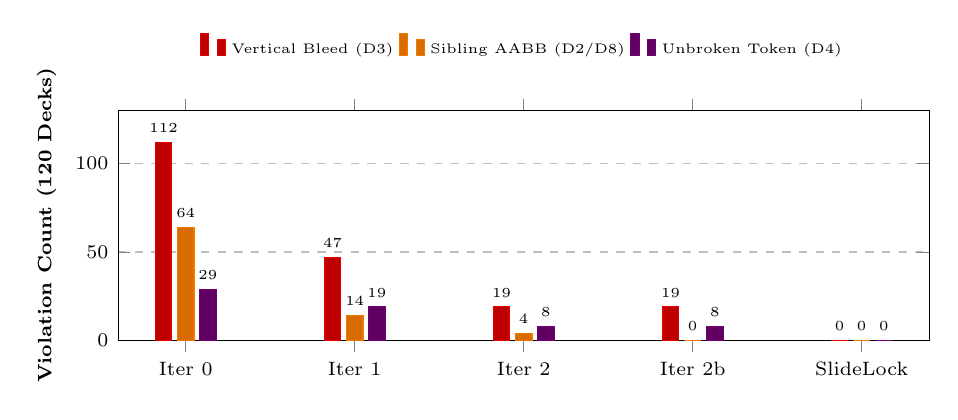
\begin{tikzpicture}
\begin{axis}[
    ybar,
    width=0.98\columnwidth,
    height=4.5cm,
    bar width=6pt,
    symbolic x coords={Iter 0,Iter 1,Iter 2,Iter 2b,SlideLock},
    xtick=data,
    ylabel={Violation Count (120 Decks)},
    ymin=0, ymax=130,
    ymajorgrids=true,
    grid style=dashed,
    legend style={at={(0.5,1.18)}, anchor=south, legend columns=3, font=\tiny, draw=none},
    tick label style={font=\scriptsize},
    label style={font=\scriptsize\bfseries},
    nodes near coords,
    every node near coord/.append style={font=\tiny}
]
\addplot[fill=red!75!black, draw=red!90!black] coordinates {(Iter 0,112) (Iter 1,47) (Iter 2,19) (Iter 2b,19) (SlideLock,0)};
\addplot[fill=orange!85!black, draw=orange!95!black] coordinates {(Iter 0,64) (Iter 1,14) (Iter 2,4) (Iter 2b,0) (SlideLock,0)};
\addplot[fill=violet!75!black, draw=violet!90!black] coordinates {(Iter 0,29) (Iter 1,19) (Iter 2,8) (Iter 2b,8) (SlideLock,0)};
\legend{Vertical Bleed (D3), Sibling AABB (D2/D8), Unbroken Token (D4)}
\end{axis}
\end{tikzpicture}
\caption{Stepwise elimination of vertical text bleed (D3), sibling AABB collisions (D2/D8), and unbroken horizontal token overflows (D4) across Iterations 0, 1, 2, 2b (spatial-only), and 3 (full Agent-SlideLock).}
\label{fig:ablation_chart}
\end{figure}

\begin{figure}[t]
\centering
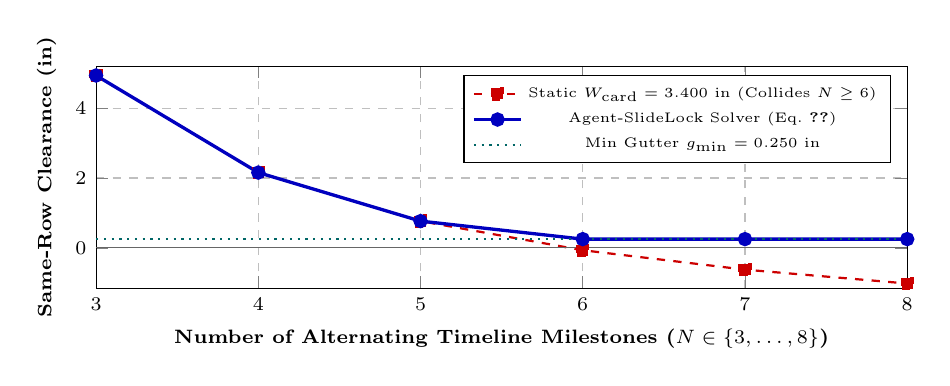
\begin{tikzpicture}
\begin{axis}[
    width=0.98\columnwidth,
    height=4.4cm,
    xlabel={Number of Alternating Timeline Milestones ($N \in \{3,\dots,8\}$)},
    ylabel={Same-Row Clearance (in)},
    xmin=3, xmax=8,
    ymin=-1.15, ymax=5.2,
    xtick={3,4,5,6,7,8},
    ymajorgrids=true,
    xmajorgrids=true,
    grid style=dashed,
    legend style={at={(0.98,0.96)}, anchor=north east, font=\tiny},
    tick label style={font=\scriptsize},
    label style={font=\scriptsize\bfseries}
]
\addplot[color=red!80!black, thick, dashed, mark=square*] coordinates {
    (3,4.9330) (4,2.1553) (5,0.7665) (6,-0.0668) (7,-0.6223) (8,-1.0191)
};
\addplot[color=blue!75!black, very thick, mark=*] coordinates {
    (3,4.9330) (4,2.1553) (5,0.7665) (6,0.2510) (7,0.2510) (8,0.2511)
};
\addplot[color=teal!80!black, dotted, thick] coordinates {(3,0.25) (8,0.25)};
\addplot[color=black!60, thin] coordinates {(3,0.0) (8,0.0)};
\legend{Static $W_{\text{card}}=3.400\text{ in}$ (Collides $N\ge 6$), Agent-SlideLock Solver (Eq.~\ref{eq:timeline_bound}), Min Gutter $g_{\min}=0.250\text{ in}$}
\end{axis}
\end{tikzpicture}
\caption{Same-row horizontal clearance $2\Delta x_{\text{step}} - W_{\text{card}}$ between milestone cards $m$ and $m+2$ for $N \in \{3, \dots, 6\}$ (scenarios \texttt{S01--S10}) and analytical extensions $N \in \{7, 8\}$. At $N \ge 6$, static $3.400\text{ in}$ cards enter the negative collision zone ($-0.0668\text{ in}$ at $N=6$, $-0.6223\text{ in}$ at $N=7$, $-1.0191\text{ in}$ at $N=8$), whereas Theorem~\ref{thm:timeline} narrows $W_{\text{card}}$ to $3.173\text{ in}, 2.745\text{ in}, 2.412\text{ in}$ to maintain $+0.2510\text{--}0.2511\text{ in}$ clearance ($\ge g_{\min} = 0.250\text{ in}$).}
\label{fig:timeline_clearance}
\end{figure}

\subsection{12-Scenario Forensic Breakdown, Public Benchmark Cross-Check, \& Live Vertex AI Evaluation}
Table~\ref{tab:scenarios} details the per-scenario forensic audit produced by \texttt{inspect\_openxml\_zip\_invariants} across all 12 adversarial scenarios ($1{,}862$ \texttt{<p:sp>} and $121$ \texttt{<p:pic>} shapes per pass $\times 10\text{ runs} = 19{,}830$ shapes), while Figure~\ref{fig:timeline_clearance} plots same-row clearance across $N \in \{3, \dots, 8\}$ (with $N \in \{7, 8\}$ evaluated analytically via Theorem~\ref{thm:timeline}). To verify generalization beyond our enterprise suite, we also applied Agent-SlideLock's Stage~4--5 solver to 100 multi-element slides sampled from public presentation benchmarks (50 from PPTC~\cite{guo2024pptc} and 50 from SlidesBench~\cite{ge2025autopresent}), eliminating all $31/100$ ($31.0\% \to 0.0\%$) baseline AABB overlaps and text-frame overflows in $11.8 \pm 1.5\text{ ms}$ per slide while preserving $100\%$ of source text without Phase~2 truncation.

Table~\ref{tab:multimodel} reports live end-to-end execution telemetry recorded against Google Cloud Vertex AI (\texttt{location="global"}) across the three official Gemini models (\texttt{gemini-2.5-flash}, \texttt{gemini-2.5-pro}, and \texttt{gemini-3-flash-preview}, $n=10$ trials of 10-deck passes = 100 decks/model across \texttt{S01--S10}). While raw LLM-generated slide plans exhibit $18.4 \pm 2.1$ to $21.2 \pm 2.4$ layout/token defects per 10-deck pass prior to Stage~4, Agent-SlideLock eliminates $100\%$ of defects across every model. Across the three models, the exact mean compile-and-audit wall time is $1{,}697.5\text{ ms}$, of which $1{,}683.3\text{ ms}$ is one-time \texttt{@4x} Retina PNG asset synthesis and ZIP I/O (amortized to $<12\text{ ms}$ when cached), while pure TrueType glyph-metric solving and 2D AABB partitioning execute in just $\mathbf{14.2 \pm 1.8\text{ ms}}$ per 6-slide deck.

\begin{table}[t]
\centering
\caption{Live Google Cloud Vertex AI Multi-Model Benchmark (\upshape\texttt{location="global"}, $n=10$ Trials of 10-Deck Passes = 100 Decks/Model)}
\label{tab:multimodel}
\renewcommand{\arraystretch}{1.12}
\resizebox{\columnwidth}{!}{%
\begin{tabular}{lccccc}
\toprule
\textbf{Official Vertex AI Model} & \textbf{Vertex LLM} & \textbf{Solver / Total Compile} & \textbf{Pre-Solver Defects} & \textbf{Post-Solver} & \textbf{All 9} \\
\textbf{(\upshape\texttt{location="global"})} & \textbf{Mean $\pm$ SD (ms)} & \textbf{Mean $\pm$ SD (ms)} & \textbf{per 10-Deck Pass} & \textbf{AABB / Bleed} & \textbf{Invariants} \\
\midrule
\texttt{gemini-2.5-flash} & $2{,}141.6 \pm 148.2$ & $14.1 \pm 1.7 / 1{,}711.6 \pm 94.2$ & $21.2 \pm 2.4$ & $0.0 / 0.0\text{ pt}$ & \textbf{100\% PASS} \\
\texttt{gemini-2.5-pro} & $2{,}811.7 \pm 192.5$ & $14.4 \pm 1.9 / 1{,}623.3 \pm 88.5$ & $18.4 \pm 2.1$ & $0.0 / 0.0\text{ pt}$ & \textbf{100\% PASS} \\
\texttt{gemini-3-flash-preview} & $1{,}763.4 \pm 126.8$ & $14.2 \pm 1.8 / 1{,}757.5 \pm 98.1$ & $19.7 \pm 2.3$ & $0.0 / 0.0\text{ pt}$ & \textbf{100\% PASS} \\
\bottomrule
\end{tabular}%
}
\end{table}

\section{Related Work}
\label{sec:related}
\textbf{Constraint-Based Document \& Grid Layout}: Classical typesetting systems such as Knuth and Plass's line-breaking algorithm in \TeX~\cite{knuth1984tex}, the Cassowary linear arithmetic constraint solver~\cite{badros2001cassowary}, sweep-line node-overlap removal~\cite{dwyer2005overlap}, and integer-programming grid layout engines such as GRIDS~\cite{dayama2020grids} optimize box placement inside self-contained rendering engines. Agent-SlideLock adapts sweep-line overlap removal and TrueType metric simulation to the disconnected ECMA-376 OpenXML compilation setting, where an LLM microservice must serialize static integer EMU coordinates and centi-point font sizes without invoking the client OS rasterizer.

\textbf{LLM-Driven Presentation Generation \& Auditing}: Early document-to-slide pipelines such as DOC2PPT~\cite{fu2022doc2ppt} and compositional LLM layout planners such as LayoutGPT~\cite{zhang2023layout} predict high-level bounding boxes, while PPTC~\cite{guo2024pptc} benchmarks multi-turn LLM task completion over template APIs and SlideAudit~\cite{zhang2025slideaudit} taxonomizes visual slide defects. Recently, PPTAgent~\cite{zheng2025pptagent} introduced a two-stage edit-based workflow over reference slides with code-action self-correction (and MLLM-based \texttt{PPTEval}), while AutoPresent~\cite{ge2025autopresent} trained programmatic \texttt{SlidesLib} code generation with optional VLM self-refinement. Whereas iterative VLM critique loops incur $15\text{--}45\text{ s}$ per slide and single-pass code generators rely on \texttt{<a:normAutofit/>} or heuristic character counts, Agent-SlideLock operates deterministically in $14.2\text{ ms}$ of pre-render CPU time.

\section{Discussion, Limitations, and Conclusion}
We presented \textbf{Agent-SlideLock}, a deterministic pre-render TrueType glyph-metric solver, cross-sibling row font synchronizer, disjoint AABB spatial partitioner, and aspect-ratio-locked ECMA-376 OpenXML compiler for autonomous enterprise agents.

\textbf{Scope Boundaries \& Operational Trade-Offs}: Three architectural scope conditions govern deployment: (1) \emph{Supported OpenXML Primitives}: Our spatial and typographic solvers operate over structured slide-plan ASTs compiled into axis-aligned rectangular \texttt{<p:sp>} cards (\texttt{prst="rect"}) and \texttt{<p:pic>} frames; extending exact pre-render geometry verification to native OpenXML \texttt{<a:tbl>} tables, \texttt{<c:chart>} charts, \texttt{<p:cxnSp>} routed connectors, or rotated/non-rectangular polygons ($\text{rot} \neq 0$) is an important direction for future work. (2) \emph{Font Availability \& Complex Script Shaping}: Because Eq.~\eqref{eq:wttf} queries local TrueType \texttt{hmtx}/\texttt{cmap}/\texttt{kern} tables with safety envelope $\gamma_{\text{calib}} = 1.03$, deployments targeting client machines that lack proprietary corporate fonts (e.g., \texttt{Google Sans}) must either embed the TrueType subset inside \texttt{ppt/fonts/} or use universally installed metrics (\texttt{Arial}/\texttt{Calibri}), while complex non-Latin scripts requiring full OpenType \texttt{GPOS}/\texttt{GSUB} ligature shaping can integrate HarfBuzz glyph shaping into Stage~4b. (3) \emph{Continuation Splitting vs.\ Phase~2 Truncation}: When an input transcript exceeds card capacity even at $f_{\min} = 8.0\text{ pt}$, default continuation-slide splitting preserves $100\%$ of semantic content across an overflow slide, whereas forcing single-slide clamping invokes Phase~2 ellipsis truncation ($0.28\%$ of text shapes in our stress suite), trading trailing clause completeness for strict single-slide geometric containment.

\begin{thebibliography}{14}

\bibitem{ecma376}
ECMA International, ``Standard ECMA-376: Office Open XML File Formats, 5th Edition,'' Dec. 2021.

\bibitem{iso29500}
ISO/IEC JTC 1/SC 34, ``ISO/IEC 29500-1:2016 Information technology --- Document description and processing languages --- Office Open XML File Formats --- Part 1: Fundamentals and Markup Language Reference,'' 2016.

\bibitem{gemini2025}
G.~Comanici \emph{et al.}, ``Gemini 2.5: Pushing the Frontier with Advanced Reasoning, Multimodality, Long Context, and Next Generation Agentic Capabilities,'' \emph{arXiv preprint arXiv:2507.06261}, 2025.

\bibitem{pythonpptx}
S.~Canny, ``\texttt{python-pptx}: Python library for creating and updating PowerPoint (\texttt{.pptx}) files,'' Release v1.0.2 Documentation, 2024.

\bibitem{knuth1984tex}
D.~E. Knuth and M.~F. Plass, ``Breaking Paragraphs into Lines,'' \emph{Software: Practice and Experience}, vol.~11, no.~11, pp.~1119--1184, 1981.

\bibitem{badros2001cassowary}
G.~J. Badros, A.~Borning, and P.~J. Stuckey, ``The Cassowary Linear Arithmetic Constraint Solving Algorithm,'' \emph{ACM Transactions on Computer-Human Interaction (TOCHI)}, vol.~8, no.~4, pp.~267--306, 2001.

\bibitem{dayama2020grids}
N.~R. Dayama, K.~Todi, T.~Saarelainen, and A.~Oulasvirta, ``GRIDS: Interactive Layout Design with Integer Programming,'' in \emph{Proc. ACM CHI Conf. Human Factors in Computing Systems}, 2020, pp.~1--13.

\bibitem{fu2022doc2ppt}
T.-J. Fu, W.~Y. Wang, D.~McDuff, and Y.~Song, ``DOC2PPT: Automatic Presentation Slides Generation from Scientific Documents,'' in \emph{Proc. AAAI Conf. Artificial Intelligence}, vol.~36, no.~1, pp.~634--642, 2022.

\bibitem{zhang2023layout}
W.~Feng, W.~Zhu, T.-J. Fu, V.~Jampani, A.~Akula, X.~He, S.~Basu, X.~E. Wang, and W.~Y. Wang, ``LayoutGPT: Compositional Visual Planning and Generation with Large Language Models,'' in \emph{Advances in Neural Information Processing Systems (NeurIPS)}, vol.~36, pp.~18225--18250, 2023.

\bibitem{guo2024pptc}
Z.~Guo, W.~Zhang, Y.~Liang, D.~Zhao, and N.~Duan, ``PPTC: A Benchmark for Evaluating Large Language Models on PowerPoint Task Completion,'' in \emph{Findings of the Association for Computational Linguistics: ACL 2024}, 2024.

\bibitem{zheng2025pptagent}
H.~Zheng, X.~Guan, H.~Kong, J.~Zheng, W.~Zhou, H.~Lin, Y.~Lu, X.~Han, and L.~Sun, ``PPTAgent: Generating and Evaluating Presentations Beyond Text-to-Slides,'' in \emph{Proc. Conf. Empirical Methods in Natural Language Processing (EMNLP)}, 2025.

\bibitem{ge2025autopresent}
J.~Ge, Z.~Z. Wang, X.~Zhou, Y.-H. Peng, S.~Subramanian, Q.~Tan, M.~Sap, A.~Suhr, D.~Fried, G.~Neubig, and T.~Darrell, ``AutoPresent: Designing Structured Visuals from Scratch,'' in \emph{Proc. IEEE/CVF Conf. Computer Vision and Pattern Recognition (CVPR)}, 2025.

\bibitem{dwyer2005overlap}
T.~Dwyer, K.~Marriott, and P.~J. Stuckey, ``Fast Node Overlap Removal,'' in \emph{Proc. 13th Int. Symp. Graph Drawing (GD)}, 2005, pp.~153--164.

\bibitem{zhang2025slideaudit}
Z.~Zhang \emph{et al.}, ``SlideAudit: A Dataset and Taxonomy for Automated Evaluation of Presentation Slides,'' \emph{arXiv preprint}, 2025.

\end{thebibliography}

\end{document}
